%図は改良の余地あり

\chapter{背景}

本章では、Multilayer~perceptron~(MLP)~及びその応用例であるGenerative~Adversarial~Networks~(GAN)~の説明を行った後にGANを画像のスタイル変換に応用したPix2pixを紹介する。

\section{MLP}

MLPは入力層と出力層を持つニューラルネットワークの一つであり、式\ref{eq:MLP}として定式化することができる。

\begin{align}
    \label{eq:MLP}
    \boldsymbol{y}&=f_{n}(W_{n}(f_{n-1}(W_{n-1}\cdots(f_{1}(W_{1}(\boldsymbol{x}))))))
\end{align}

ここで、$\boldsymbol{x}$はMLPへの入力の教師データ,$\hat{\boldsymbol{y}}$はMLPの出力,$\boldsymbol{y}$はMLPの出力の教師データ,$n$は層の総数,$f_{i}$は$i$番目の層の活性化関数,$W_{i}$は$i$番目の層の重みの行列である。

%ここの誤差逆伝播をもう少し詳しく書くか?
また、損失関数$L(\hat{\boldsymbol{y}},\boldsymbol{y})$を小さくする方向に重みの更新が行われることで学習は進むが、任意の活性化関数が微分可能である時は誤差逆伝播法により高速に重みの更新を行うことが可能である。

\section{GAN}

\begin{figure}[t]
\begin{center}
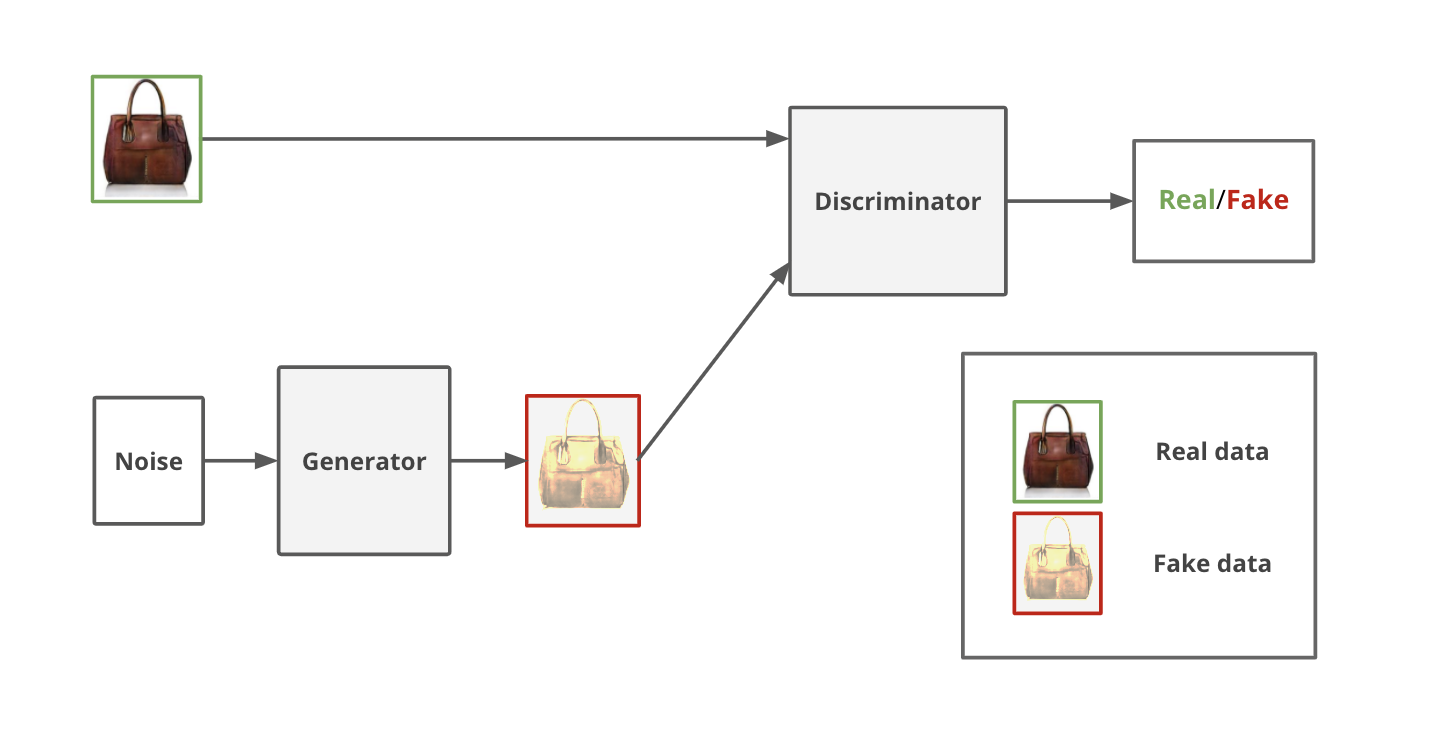
\includegraphics[width=\hsize]{figure/GAN_net.png}
\caption{GANのネットワークの図}
\label{fig:GAN_net}
\end{center}
\end{figure}


GAN~\cite{GAN}はMLPの応用例であり、生成モデルと識別モデルが競合して学習を行う。生成モデルは自身の出力が学習データであると識別モデルに推定させること、識別モデルは学習データと生成モデルの出力のどちらであるかを識別することを目指して学習する。

また、生成モデルの目的関数は式\ref{eq:GAN_G}であり、識別モデルの目的関数は\ref{eq:GAN_D}である。

\begin{align}
    \label{eq:GAN_G}
    \argmin _{\theta_G}& \mathbb{E}_{\boldsymbol{z}}[\log (1-D(G(\boldsymbol{z};\theta_G);\theta_D))]\\
    \label{eq:GAN_D}
    \argmax _{\theta_D}& \mathbb{E}_{\boldsymbol{x}}[\log D(\boldsymbol{x};\theta_D)]+\mathbb{E}_{\boldsymbol{z}}[\log (1-D(G(\boldsymbol{z};\theta_G);\theta_D))]
\end{align}

ここで、$\boldsymbol{x}$は学習データ,$\boldsymbol{z}$は生成モデルへの入力のノイズ,$G(\boldsymbol{z};\theta_G)$はノイズ$\boldsymbol{z}$を入力とする生成モデル,$D(\cdot;\theta_D)$は識別モデル,$\theta_G$は生成モデル$G$のパラメータ,$\theta_D$は識別モデル$D$のパラメータである。



\section{Pix2pix}

\begin{figure}[t]
\begin{center}
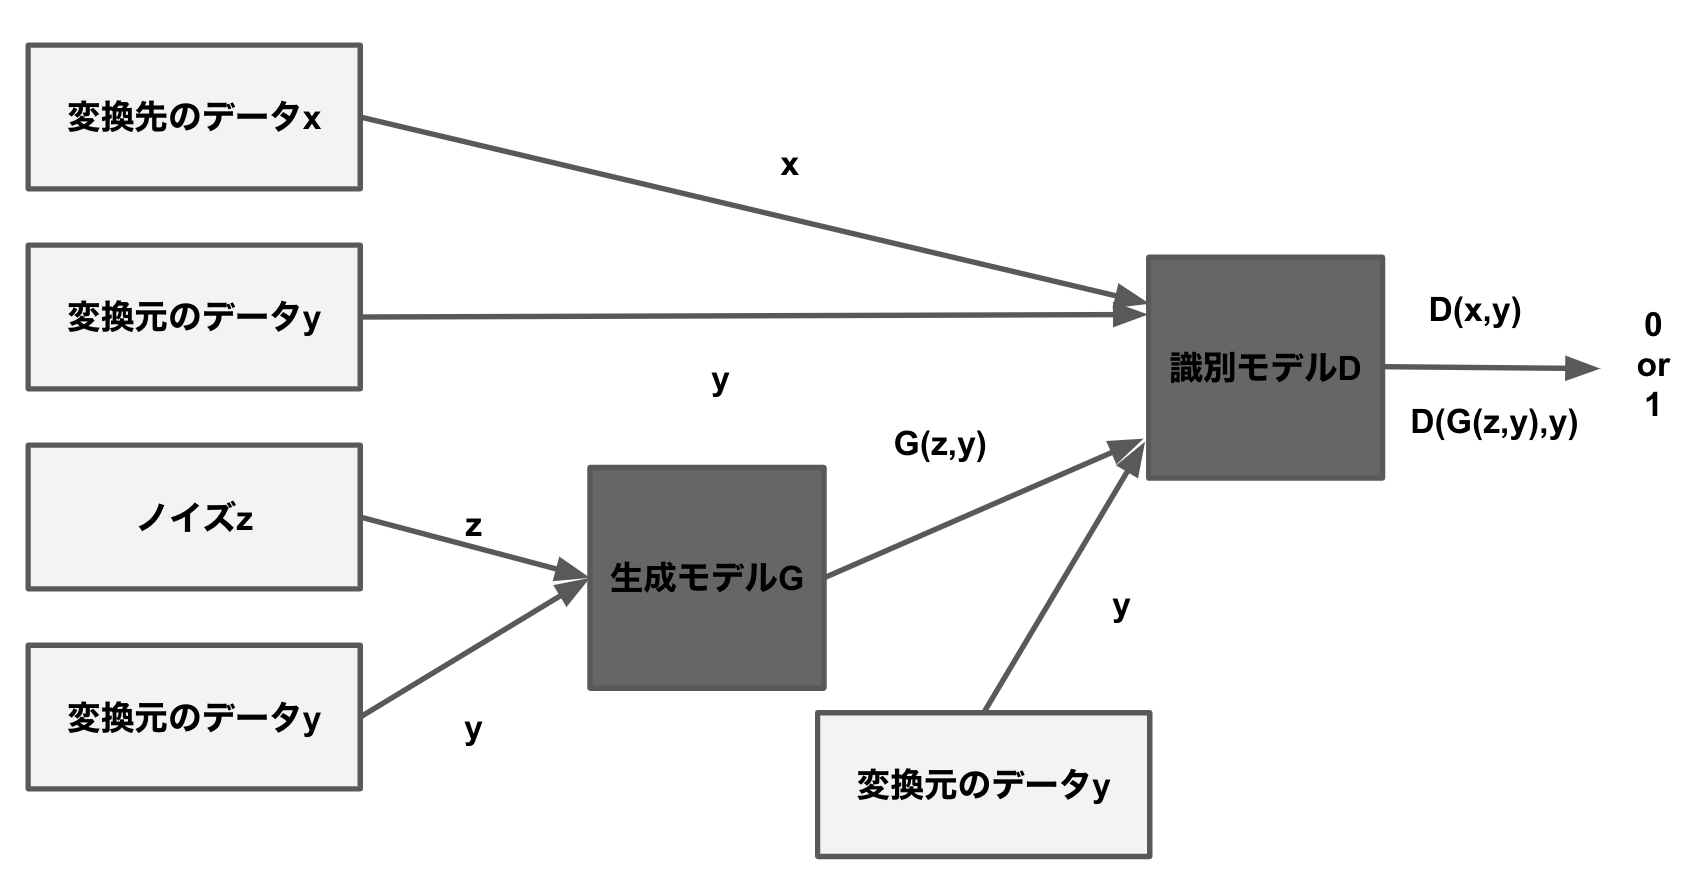
\includegraphics[width=\hsize]{figure/pix2pix_net.png}
\caption{pix2pixのネットワークの図}
\label{fig:pix2pix_net}
\end{center}
\end{figure}

Pix2pix~\cite{pix2pix}はある条件下で画像間の変換を行うGANである。図\ref{fig:pix2pix_img}にあるようにピクセルの対応関係を変えずにスタイル変換を行うことができる。

\begin{figure}[t]
\begin{center}
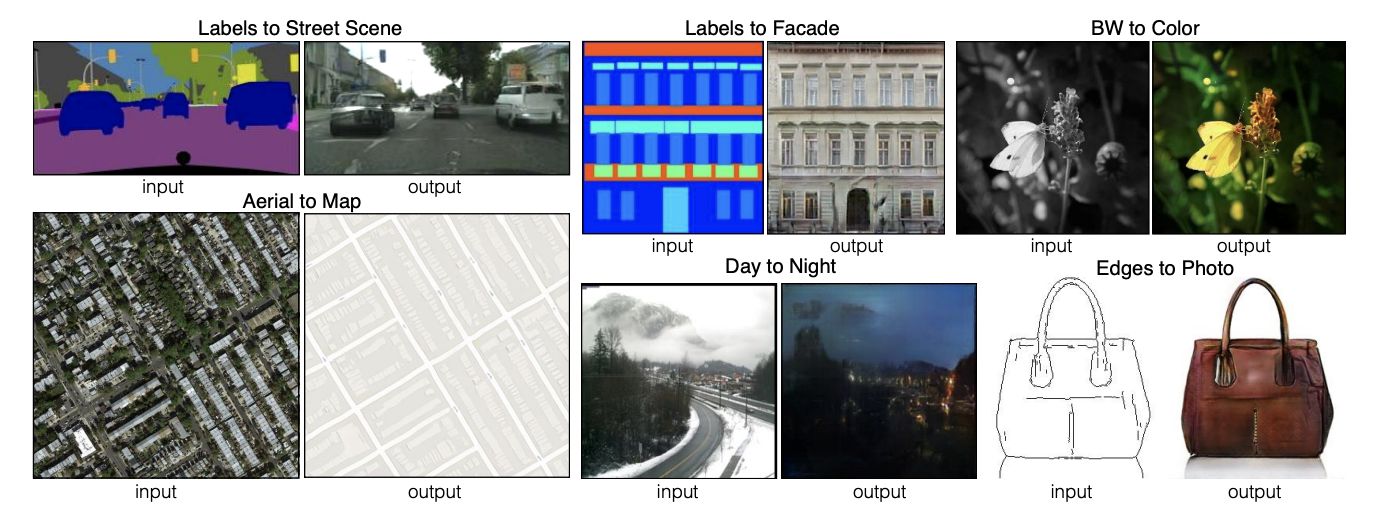
\includegraphics[width=\hsize]{figure/pix2pix_img.png}
\caption{pix2pixのスタイル変換の例}
\label{fig:pix2pix_img}
\end{center}
\end{figure}

また、生成モデルの目的関数は式\ref{eq:pix2pix_G}であり、識別モデルの目的関数は\ref{eq:pix2pix_D}である。このような条件付きのGANをConditional~GAN~\cite{CGAN}と呼ぶ。

\begin{align}
    \label{eq:pix2pix_G}
    \argmin _{\theta_G}& \mathbb{E}_{\boldsymbol{x}, \boldsymbol{z}}[\log (1-D(\boldsymbol{x}, G(\boldsymbol{x}, \boldsymbol{z}; \theta_G); \theta_D))]+\mathbb{E}_{\boldsymbol{x}, \boldsymbol{y}, \boldsymbol{z}}[\|\boldsymbol{y}-G(\boldsymbol{x}, \boldsymbol{z}; \theta_G)\|_{1}]\\
    \label{eq:pix2pix_D}
    \argmax _{\theta_D}& \mathbb{E}_{\boldsymbol{x}, \boldsymbol{y}}[\log D(\boldsymbol{x}, \boldsymbol{y}; \theta_D)]+\mathbb{E}_{\boldsymbol{x}, \boldsymbol{z}}[\log (1-D(\boldsymbol{x}, G(\boldsymbol{x}, \boldsymbol{z}; \theta_G); \theta_D))]
\end{align}


ここで、$\boldsymbol{x}$は変換先の学習データ,$\boldsymbol{y}$は変換元の学習データ,$\boldsymbol{z}$は生成モデルへの入力のノイズ,$G(\boldsymbol{x},\boldsymbol{z};\theta_G)$はノイズ$\boldsymbol{z}$を入力とする生成モデル,$D(\boldsymbol{x},\cdot;\theta_D)$は識別モデル,$\theta_G$は生成モデル$G$のパラメータ,$\theta_D$は識別モデル$D$のパラメータである。

\subsection{生成モデルの構造}

\begin{figure}[t]
\begin{center}
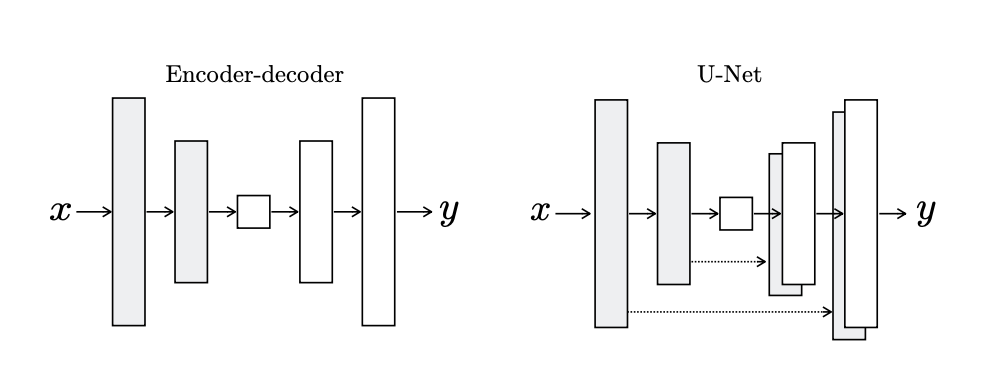
\includegraphics[width=\hsize]{figure/u-net.png}
\caption{U-netのネットワーク}
\label{fig:u-net}
\end{center}
\end{figure}

スタイル変換では基礎的な構造を保持したまま変換を行う必要があり、一般にはencoder-decoderのネットワークが用いられる。Pix2pixの生成モデルでは、\ref{fig:u-net}のようにU-net\cite{u-net}で用いられるスキップコネクションを持ったネットワークを用いている。

\subsection{識別モデルの構造}

Pix2pixの識別モデルでは、局所的な部分の識別の精度を高めるためにPatchGANという手法を用いている。これにより、パッチと呼ばれる小領域ごとで学習データであるかどうかの識別を行うことができる。


